\documentclass[xcolor=dvipsnames]{beamer}
\useoutertheme{infolines}
\setbeamertemplate{navigation symbols}{}
\setbeamertemplate{items}[ball]
\usepackage{graphicx,multirow,color,xcolor,verbatim,float,comment,amsmath}
\setbeamertemplate{frametitle}[default][center]
\begin{document}
\title{Simultaneously Identifying Multiple Pathways with Alternative Scoring Criteria}
\author{Bowen Deng}
\institute{Dept. of Prob. and Stat.}
\date{}
\begin{frame}
\maketitle
\end{frame}
\section{Organization}
\begin{frame}
We'll discuss in the following aspects:\\
\begin{itemize}
\item Simultaneously Detection of Multiple Pathways with Alternative Scoring Criteria\\
\item Danger in Simulation Study\\
\item Difficulty in Stability Criteria\\
\item Further Work
\end{itemize}
\end{frame}
\section{Simultaneous Pathway Detection with Alternative Scoring Criteria}
\subsection{Literature Review}
\begin{frame}{Simultaneously Detecting Multiple Pathways}
Objective:
\begin{displaymath}
\begin{split}
\max O(M_1,\cdots,M_t)&=\sum_{i=1,\cdots,t} W(M_i)\\
s.t. |M_i|&\in[k_{\min},k_{\max}]\\
M_i\cap M_j&=\emptyset
\end{split}
\end{displaymath}
Greedy approach: Iteratively find maximizer $\hat{M_i},i=1,\cdots,t$ of $W(M)$.
\end{frame}
\begin{frame}{Integer Linear Programming}
\begin{displaymath}
\begin{split}
\max O(M_1,\cdots,M_t)=\sum_{\rho=1}^t\sum_{i=1}^m(2C_i(M_{\rho})&-\sum_{j=1}^nI_{M_{\rho}}(j)A_{ij})\\
s.t. \sum_{j=1}^nI_{M_{\rho}}(j)A_{ij}&\geqslant C_i(M_{\rho})\\
\sum_{\rho=1}^tI_{M_{\rho}}(j)&\leqslant 1\\
k_{\min}\leqslant \sum_{j=1}^nI_{M_{\rho}}(j)&\leqslant k_{\max}
\end{split}
\end{displaymath}
\end{frame}
\begin{frame}
\begin{figure}
\centering
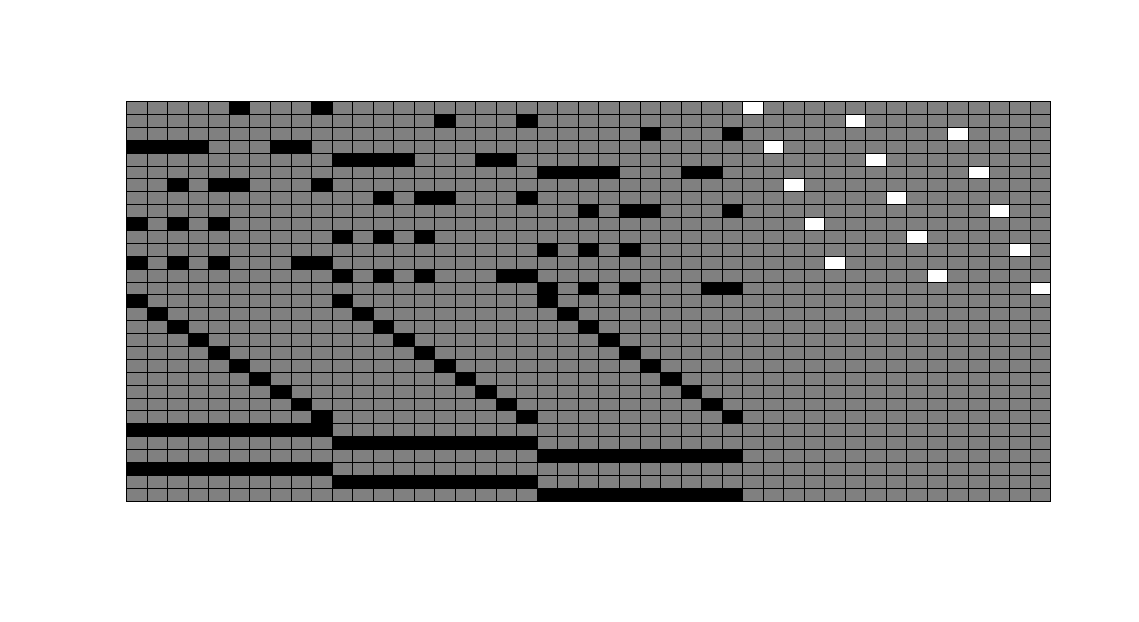
\includegraphics[width=0.9\linewidth]{ILP.png}
\caption{The coefficients of the ILP}
\end{figure}
\end{frame}
\begin{frame}{MDendrix and IterDendrix}
To find $t$ pathways, one method is to solve the ILP directly. (MDendrix)\\
Another iterative approach is to solve the ILP with $t=1$, delete the identified genes, and run iteratively. (iterDendrix)\\
By theory, the time cost of MDendrix and iterDendrix is comparable with small $t$.\\
\begin{displaymath}
\begin{split}
TC(M)&\geqslant TC(\text{iter once})\\
&=\frac{\sum_{\rho=1}^tTC(\text{iter once})}{t}\\
&=\frac{TC(\text{iterDendrix})}{t}\\
&\geqslant \frac{TC(\text{mDendrix})}{t}
\end{split}
\end{displaymath}
\end{frame}
\begin{frame}
The authors used CPLEX v12.3 for implementation. We use lpSolve package in R. Set simulation data with $m=200$, $n=1000$, $I=10$, $t=3$. $k_{\min}=8$, $k_{\max}=12$.\\
MDendrix:\\
\begin{displaymath}
\begin{array}{ccc}
\text{Time Cost}&184.32&\\
\text{Result}&\text{Score}&\text{Score of Standard}\\
1\sim 10\,761\,774&30&32\\
11\sim 20\,752\,973&35&40\\
21\sim 30\,34\,109&32&36\\
\end{array}
\end{displaymath}
IterDendrix:\\
\begin{displaymath}
\begin{array}{ccc}
\text{Time Cost}&7.06&\\
\text{Result}&\text{Score}&\text{Score of Standard}\\
1\sim10\,214\,774&30&32\\
21\sim 30\,34\,109&32&36\\
11\sim 20\,652\,752&35&40
\end{array}
\end{displaymath}
\end{frame}
\subsection{Candidate Criteria}
\begin{frame}{Candidate Criteria}
For mutation matrix $A$, $p$ takes value in $m$ patients, and $g$ takes value in $n$ genes. $M$ is a set of genes.\\
We borrow the criteria from RME, an alternative approach for driver pathway identification.\\
Coverage Score:\\
\[C(M)=\frac{\#(\exists g\in M \text{ mutates in }p)}{m}\]
Exclusivity Score:\\
\[E(M)=\frac{\#(\text{exactly one } g\in M \text{ mutates in }p)}{\#(\exists g\in M \text{ mutates in }p)}\]
\end{frame}
\begin{frame}
Denote $I_M(p)$ the occurrence indicator of mutations of patient $p$ in $M$.\\
\begin{equation}
\begin{split}
S(M)&=C(M)+E(M)\\
&=\frac{\#\{I_M(p)>0\}}{m}+\frac{\#\{I_M(p)=1\}}{\#\{I_M(p)>0\}}\\
W(M)&=2\#\{I_M(p)>0\}-\sum_pI_M(p)\\
\end{split}
\end{equation}
The objective is to find $\hat{M}$ as the maximizer of $S(M)$. We could also restrict $|M|=k$.\\
\end{frame}
\begin{frame}{Properties of New Criteria}
\begin{itemize}
\item The score is fixed for patients who has mutations in the gene set.\\
\item Fixing coverage, $E(M)$ promotes more ones.\\
\item Fixing $\#\{I_M(p)=1\}$, coverage tends to obtain either extreme: whole coverage or all ones.\\
\end{itemize}
\end{frame}
\begin{frame}{Simultaneous Detection with New Criteria}
We combine this new criteria with mDendrix to detect a mutually exclusive set of genes $M=\{M_1,\cdots,M_t\}$ which maximizes:
\[
S(M)=\sum_{\rho=1}^t S(M_{\rho})
\]
$k_{\min}\leqslant |M_{\rho}|\leqslant k_{\max}$.\\
\end{frame}
\subsection{Multiple Value Genetic Algorithm}
\begin{frame}{Computation}
The objective is to maximize $S(M)$. GA (Genetic Algorithm) is one of the top choices:\\
\begin{itemize}
\item The problem is no longer an ILP (Integer Linear Programming) task.\\
\item MCMC might trap in a local maxima.\\
\item The return value of GA is a set of solutions, suboptimal solutions are obtained as bonus.\\
\item GA's time cost is tractable.\\
\item GA is flexible for further integrated approach and variable scoring settings.\\
\end{itemize}
However, we should generalize the GA because it only works for binary case.\\
\end{frame}
\begin{frame}{Multiple Value Genetic Algorithm}
\begin{figure}
\centering
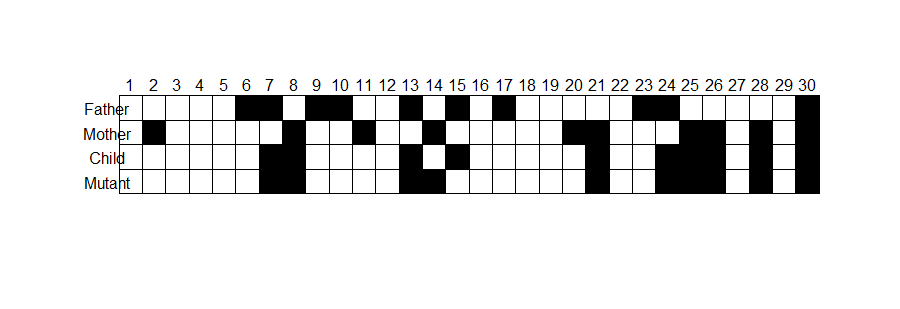
\includegraphics[width=0.9\linewidth]{GA.png}
\caption{Genetic Algorithm with $0-1$ values}
\end{figure}
We generalize GA to MVGA (Multiple Value Genetic Algorithm), it is analogous to the GA.\\
\end{frame}
\begin{frame}{Review of GA}
\begin{itemize}
\item Select a population\\
\item Crossproduct\\
\item Mutation\\
\item Form a new population
\end{itemize}
However, the crossproduct should deal with multiple value vectors rather than $0-1$ vectors.\\
\end{frame}
\begin{frame}{Toy Example of GA}
We would like to maxmize $f(x)=e^{-x^2}, x\in[-5,5]$.\\
\begin{figure}
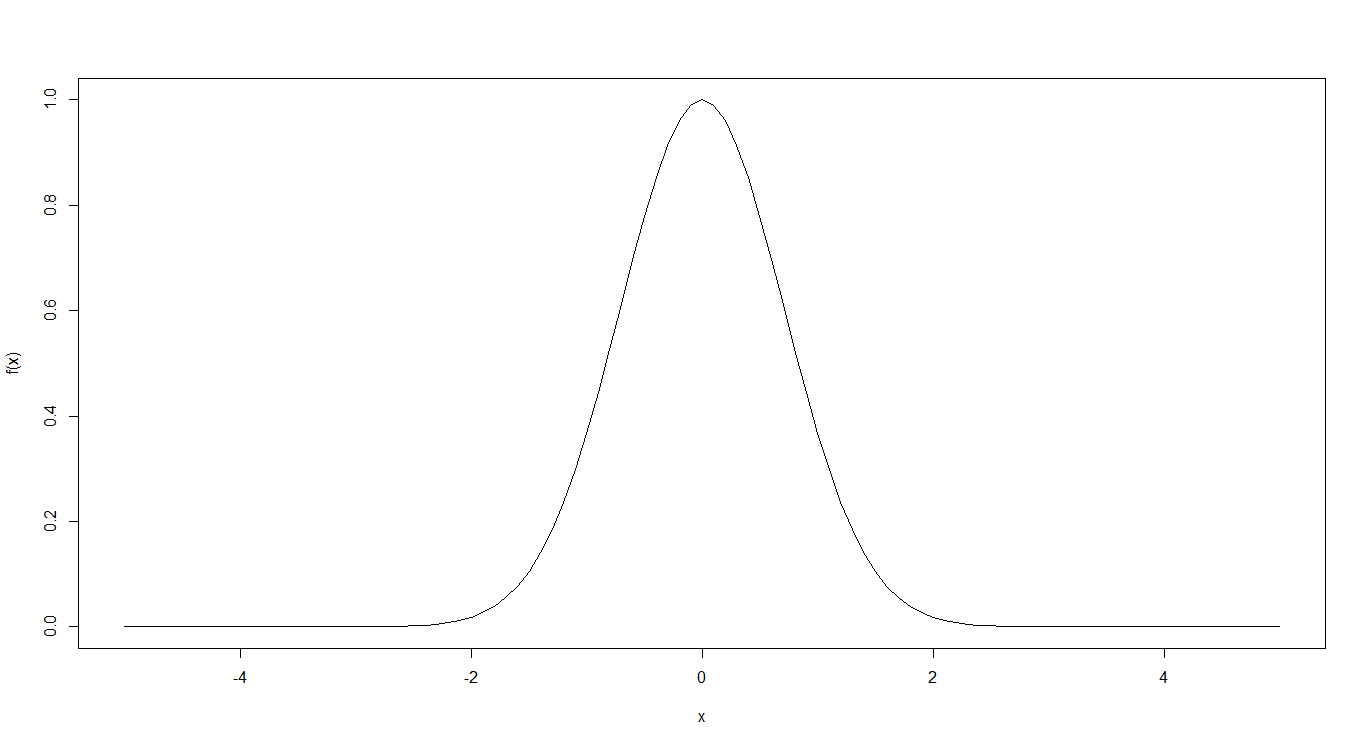
\includegraphics[width=0.9\linewidth]{toyfunction.png}
\caption{Objective Function}
\end{figure}
\end{frame}
\begin{frame}{Select Population}
We first select a parent generation of size 10 from $[-5,5]$.\\
2.42  2.33  2.04  2.00 -0.71  1.16 -1.16  1.75  3.66  4.20\\
We calculate $f(x)$ for these parents:\\
2.75e-03 4.22e-03 1.51e-02 1.79e-02 5.99e-01 2.58e-01 2.59e-01 4.66e-02 1.47e-06 2.01e-08\\
We select two of the parents to produce a child.\\
The probability of $x$ being selected is proportional to $f(x)$, therefore, an elite is more likely to be chosen than a normal person candidate.\\
The crossproduct is flexible with specific problems, here we could use $cp(x,y)=\frac{x+y}{2}$.\\
For example, the parents are -0.715157  1.163802, the child is 0.22.\\
\end{frame}
\begin{frame}{Crossproduct}
With probability 0.1, the child might mutate.\\
For example, 0.22 might mutate to 0.21 or 0.23 if the score could be higher.\\
In this case, 0.22 will mutate to 0.21.\\
After ten productions, we get ten parents and ten children.\\
Parents:\\
2.42  2.33  2.04  2.00 -0.71  1.16 -1.16  1.75  3.66  4.20\\
Children:\\
-0.9384129 -0.9384129  0.2243223 -0.9384129  0.2243223  0.8115732  0.2243223 -0.9384129 -0.9384129 -0.9384129
\end{frame}
\begin{frame}{Iteration}
We pool the parents and the children and get 20 candidates.\\
We remain the 10 top scored ones.\\
0.2243223 -0.7151570  0.8115732 -0.9384129 -1.1616687  1.1638017  1.7504537  2.0054783  2.0472774  2.3383034 2.4277411  3.6646631  4.2097401\\
We use them to produce the next generation iteratively until convergence.\\
-7.244348e-09  5.279007e-09  2.856562e-10 -9.826706e-10 -5.023779e-09 -3.485072e-10 -7.144341e-09  4.050658e-09  2.782331e-09 6.547334e-09\\
\end{frame}
\begin{frame}{Crossproduct}
Denote father: $a_1,\cdots,a_n$, $b_1,\cdots,b_n$, $a_i,b_i\in\{0,1,\cdots,t\}$.\\
$a_i=\rho$ means i-th gene is in the $\rho$-th set, if $\rho=0$, i-th gene is not selected.\\
The motivation is to find a feasible solution corresponding to child $c_1,\cdots,c_n$ under constraint:\\
\[
\sum_{i=1}^n[(1-x_i)I(a_i=\rho)+x_iI(b_i=\rho)]\in[k_{\min},k_{\max}]
\]
where $x_i=0$ represents $c_i=a_i$, and $x_i=1$ represents $c_i=b_i$.\\
We also wish the child to deviates from the parents so that $\sum_ix_i\approx \frac{n}{2}$.\\
Therefore, we would like to maximize $\sum_ix_i$, with constraint $\sum_ix_i\leqslant \frac{n}{2}$.\\
\end{frame}
\subsection{Parameter Selection}
\begin{frame}{Selection of $k_{\min}$ and $k_{\max}$}
The hunt for an appropriate $k$ not only meets difficult in theory but also deviates results in simulation study.\\
Theoretically, the peak value often takes at $l=k\pm 1$ rather than exact $k$.\\
Practically, the overlapping criteria is not unimodal and unstable with small $t$.\\
On the other hand, large $t$ is computationally expensive.\\
Moreover, biologically speaking, we should not restrict ourselves to one certain $k$.\\
We could try estimating the bound of $k$: $k_{\min}$ and $k_{\max}$.\\
It would make much more sense.\\
\end{frame}
\begin{frame}
The idea is that for appropriate $k_{\min}$ and $k_{\max}$, the length of $M_1,\cdots,M_t$ should be dispersed in $[k_{\min},k_{\max}]$ uniformly.\\
Therefore, we follow the procedure to search for the best $k_{\min}, k_{\max}$.\\
\begin{figure}
\centering
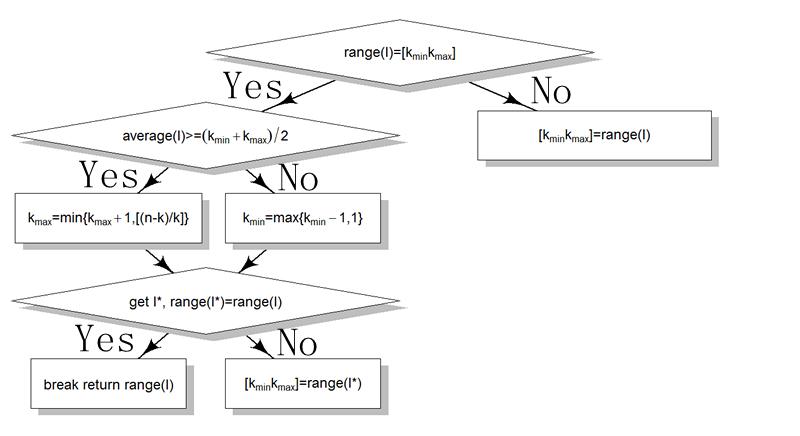
\includegraphics[width=\linewidth]{selection.png}
\end{figure}
\end{frame}
\begin{frame}{Toy Example}
Suppose we would like to find
\begin{displaymath}
\begin{split}
(x_1,x_2,\cdots,x_{10})&=\arg\min O(\vec{x})\\
&=\sum_{i=1}^5(x_i-4)^2+\sum_{i=6}^{10}(x_i-6)^2\\
s.t. k_{\min}\leqslant &x_i\leqslant k_{\max}
\end{split}
\end{displaymath}
\end{frame}
\begin{frame}
The ideal $k_{\min}=4$, $k_{\max}=6$.\\
Take initial $k_{\min}=3$, $k_{\max}=5$, the iteration runs as the following:\\
\begin{itemize}
\pause
\item $k_{\min}=3,k_{\max}=5$
\item 4,4,4,4,4,5,5,5,5,5\\
\pause
\item $k_{\min}=4, k_{\max}=5$\\
\item 4,4,4,4,4,5,5,5,5,5\\
\pause
\item $k_{\min}=3,k_{\max}=6$\\
\item 4,4,4,4,4,6,6,6,6,6\\
\pause
\item $k_{\min}=4,k_{\max}=6$\\
\item 4,4,4,4,4,6,6,6,6,6\\
\pause
\item $k_{\min}=3,k_{\max}=7$\\
\item 4,4,4,4,4,6,6,6,6,6\\
\pause
\end{itemize}
Therefore, the best $k_{\min}=4$, $k_{\max}=6$.\\
\end{frame}
\section{Danger in Simulation Study}
\begin{frame}{Independence Gene Model (IGM)}
Let $A$ be an $m\times n$ mutation matrix so that $\hat{M}$ is a submatrix of $A$ and $|\hat{M}|=k$.\\
IGM conditions:\\
1. Each gene $g\notin \hat{M}$ is mutated independently in each patient with probability $p_g\in[p_L,p_U]$. (Low rate passenger mutation)\\
2. $W(\hat{M})=rm$. (Average row score $r$)\\
3. $\forall l$, any subset $M\subset \hat{M}$ of cardinality $|M|=l$ satisfies: $W(M)\leqslant \frac{l+d}{k}W(\hat{M})$, for a constant $0\leqslant d<1$. (No dominant submatrix)\\
IGM is a standard assumption for somatic single nucleotide mutations.\\
The genes in $\hat{M}$ are modelled to be the driver pathway.\\
\end{frame}
\begin{frame}{Generation of Simulation Data}
In our study, we often use the following simulation data based on IGM requirements.\\
Mutation matrix $A$ is constructed as following:\\
\begin{itemize}
\item The top $I\cdot t$ columns represent $t$ groups of driver genes, each group contains $I$ genes.\\
\item For each group, we set the row sums follows a distribution concentrating at 1. (e.g. $p(x)=(0.9-0.85|x-1|)^+$)\\
\item For other genes, we consider them as passenger genes which mutates with probability $p_m=O(1/m)$.\\
\end{itemize}
\end{frame}
\begin{frame}{The Reason for Failure}
Take WMSP problem as an example, if we want to select $k\in[k_{\min},k_{\max}]$ columns such that the submatrix $M$ obtains maximum $W(M)$.\\
We first select the top $k$ columns $M_0$. Suppose the patients mutated in $M_0$ are $\Gamma(M)\subset \{1,\cdots,m\}$. Consider an outsider gene $g$, an insider gene $g_0$, such that $W(M\setminus \{g_0\})\triangleq W(M')\geqslant \frac{k-1}{k}W(M)$.\\
\begin{displaymath}
\begin{split}
W(M'\cup \{g\})&=W(M')+\#\{\text{patients mutated in }g\text{, but not in }\Gamma(M')\}\\
&\phantom{=W(M)'}-\#\{\text{patients mutated in both }g\text{ and }\Gamma(M')\}\\
&\triangleq W(M')+|\Gamma(g)\setminus\Gamma(M')|-|\Gamma(g)\cup\Gamma(M')|\\
&\geqslant \frac{k-1}{k}W(M)+|\Gamma(g)\setminus\Gamma(M')|-|\Gamma(g)\cup\Gamma(M')|
\end{split}
\end{displaymath}
\end{frame}
\begin{frame}
Denote $x_i=I\{i\in\Gamma(g)\}$. Assume $\Gamma(M')=\{1,\cdots,m_0\}$, $m_0<m$, $m-m_0\ll m$.\\
\begin{displaymath}
\begin{split}
\Pr(\omega_g)&= \Pr(W(M'\cup\{g\})>W(M))\\
&\geqslant\Pr(|\Gamma(g)\setminus\Gamma(M')|-|\Gamma(g)\cup\Gamma(M')|>\frac{W(M)}{k})\\
&=\Pr(x_{m_0+1}+\cdots+x_{m}>x_1+\cdots+x_{m_0}+r)\\
&=\Pr(Y>Z+r) (\text{where }Y\sim B(m-m_0,p), Z\sim B(m_0,p))\\
\end{split}
\end{displaymath}
where $r$ is the density of $M$: $W(M)=rm$.\\
Numerically, if $p=0.01$, $m=100$, $m_0=95$, $n=1000$, $r=0.9$, the probability $\Pr(\omega_g)>0.02$.\\
\[\Pr(\cup_g\omega_g)\approx 1\]
\end{frame}
\begin{frame}{Conclusion}
With high probability, the submatrix found that maximize $W(M)$ contains passenger genes.\\
The accuracy of the methods could not be calculated only by its symmetric difference (or other similar criterion) with expected result ($1,\cdots,10$ in our case).\\
We could actually use Brute Force strategy to get the optimal solution for smaller datasets, and use these results as a ruler.\\
\end{frame}
\section{Selection of $k$ via Stability Criteria}
\begin{frame}{Motivation}
We would like to select the $l$ important genes from all genes $A=\{1,2,\cdots,n\}$, when the true pathway gene set is $\hat{M}=\{1,2,\cdots,k\}$.\\
If $l\neq k$, the result would be unstable. Therefore, we would like to build a criteria to determine the $l$ without prior knowledge on $k$.
\end{frame}
\begin{frame}{Model}
The idea is to abstract the result from the IGM (Independence Gene Model). We set a probability model for the result gene set.\\
Denote $\vec{x}=(x_1,\cdots,x_n)$ the indicator vector for $M\subset A$, $|M|=l$.\\
Assume the distribution $\triangleq M(n,k,l)$:
\[
f(\vec{x})=p^{x_{k+1}+\cdots +x_n}/A(n,k,l)
\]
where $p=O(1/n)$.\\
\[
A(n,k,l)=\sum_{u}C_k^uC_{n-k}^{l-u}p^{l-u}
\]
\end{frame}
\begin{frame}{Problem}
Run pairs of results $I_i,J_i\stackrel{i.i.d.}{\sim} M(n,k,l), i=1,2,\cdots, t$.\\
We would like to estimate EOS (Expectation of Overlapping Size) defined as:
\[C(l)=\frac{\sum_{i=1}^t|I_i\cap J_i|}{t}\]
By LLN (Law of Large Numbers), $C(l)\approx\mathbb{E}C(l)=\mathbb{E}|I_1\cap J_1|.$\\
After calculations, the problem reduces to\\
\begin{displaymath}
\begin{split}
C(l)&\approx \mathbb{E}|I_1\cap J_1|\\
&=k(\frac{A(n-1,k-1,l-1)}{A(n,k,l)})^2+(n-k)(p\frac{A(n-1,k,l-1)}{A(n,k,l)})^2
\end{split}
\end{displaymath}
\end{frame}
\begin{frame}{Simulation Study}
\begin{figure}
\centering
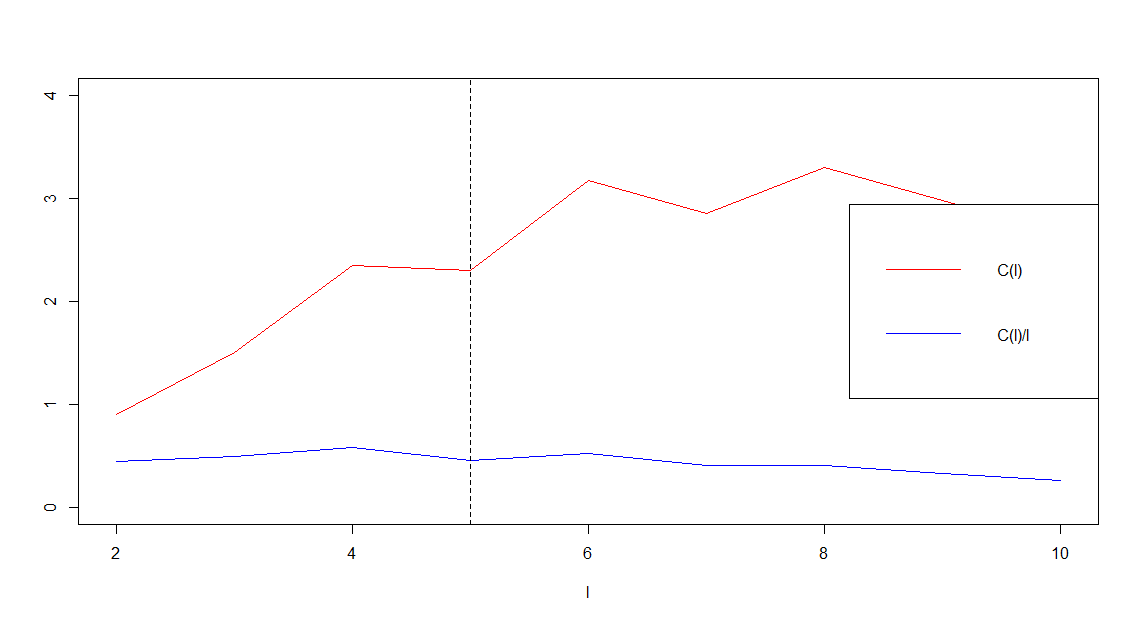
\includegraphics[width=0.9\linewidth]{overlapcrit.png}
\caption{The relation of $l$ and average of $C(l)$ for 10 tests, simulated data of 50 patients, 200 genes, 5 driver mutation genes}
\end{figure}
\end{frame}
\begin{frame}
With the settings in the simulation data, the mutation rate in the model $p$ should be $0.1$.\\
\begin{figure}
\centering
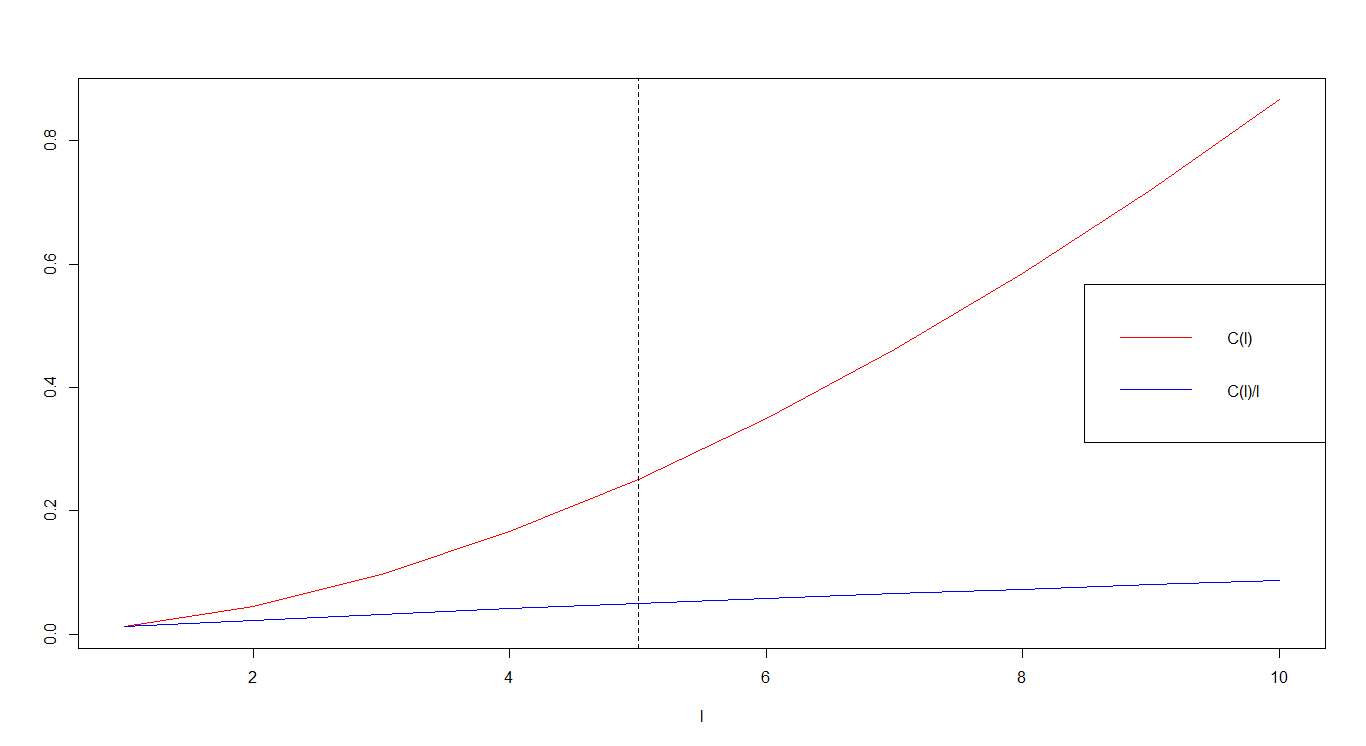
\includegraphics[width=0.9\linewidth]{theorycover.png}
\caption{$\mathbb{E}C(l)$ with respect to $l$, where $p=0.1$, $n=200$, $k=5$}
\end{figure}
\end{frame}
\begin{comment}
\begin{frame}
\begin{table}
\begin{tabular}{ccc}
$l$&$|I_1\cup I_2|$&mean\\
\hline
\multirow{2}{*}{3}&0 1 2 3&\multirow{2}{*}{1.5}\\
&3 17 17 3&\\
\multirow{2}{*}{4}&0 1 2 3 4&\multirow{2}{*}{2.35}\\
&1 6 14 16 3&\\
\multirow{2}{*}{5}&0 1 2 3 4 5&\multirow{2}{*}{2.3}\\
&1 9 14 10 5 1&\\
\multirow{2}{*}{6}&0 1 2 3 4 5 6&\multirow{2}{*}{3.175}\\
&3 10 13 6 7 1&\\
\multirow{2}{*}{7}&1 2 3 4 5&\multirow{2}{*}{2.85}\\
&6 12 7 12 3&\\
\multirow{2}{*}{8}&1 2 3 4 5 7&\multirow{2}{*}{3.3}\\
&2 10 11 10 6 1&\\
\multirow{2}{*}{9}&1 2 3 4 5 6&\multirow{2}{*}{2.975}\\
&5 14 8 6 4 3&\\
\multirow{2}{*}{10}&1 2 3 4 5&\multirow{2}{*}{2.65}\\
&8 13 9 5 5&\\
\hline
\end{tabular}
\end{table}
\end{frame}
\end{comment}
\section{Further Work}
\begin{frame}{Further Study Directions}
\begin{itemize}
\item Find better crossproduct method for MVGA\\
\item Use both simulation data and biological data to test the new method\\
\item Selection of $t$ in simultaneous identification\\
\item Mathematically prove the reliability of parameter selection of $k_{\min}$ and $k_{\max}$\\
\item Illustration of the reason why candidate scoring scheme is preferable\\
\end{itemize}
\end{frame}
% Inspired by RME, for the sake of computational efficiency, we should filter out genes with small recurrence.\\
\end{document}
